\documentclass[12pt]{article}
\usepackage[margin=1in]{geometry}
\usepackage{amsmath,amssymb,booktabs,graphicx,natbib,hyperref,placeins}
\renewcommand{\topfraction}{0.95}
\renewcommand{\bottomfraction}{0.95}
\renewcommand{\textfraction}{0.05}
\renewcommand{\floatpagefraction}{0.7}
\hypersetup{colorlinks=true,linkcolor=blue,citecolor=blue,urlcolor=blue}
\graphicspath{{figures/}}
\newcommand{\R}{\mathbb{R}}
\newcommand{\cut}{\mathcal{C}}
\newcommand{\nnl}{\operatorname{NNL}}
% Generated from verified current-version observations.
\newcommand{\CurrentCases}{191}
\newcommand{\CurrentInfeasible}{8}
\newcommand{\CurrentLargeCpuSeconds}{243.9}
\newcommand{\CurrentLargeCpuMinutes}{4.1}
\newcommand{\CurrentLargeCpuMemory}{58.8}
\newcommand{\CurrentLargeNearest}{0.618}
\newcommand{\CurrentPlainFidelity}{0.0070}
\newcommand{\CurrentPlainHighRankFidelity}{0.0027}
\newcommand{\CurrentPowerFidelity}{0.1367}
\newcommand{\CurrentPowerHighRankFidelity}{0.0936}
\newcommand{\CurrentPlainGlobal}{0.625}
\newcommand{\CurrentPlainNearest}{0.369}
\newcommand{\CurrentCombinedGlobal}{0.706}
\newcommand{\CurrentCombinedNearest}{0.282}
\newcommand{\CurrentGraphGlobal}{0.791}
\newcommand{\CurrentGraphNearest}{0.254}
\newcommand{\CurrentNativeGlobal}{0.666}
\newcommand{\CurrentNativeNearest}{0.274}
\newcommand{\CurrentMatchedGlobal}{0.577}
\newcommand{\CurrentMatchedNearest}{0.346}
\newcommand{\CurrentMatchedGroupsGlobal}{0.668}
\newcommand{\CurrentMatchedGroupsNearest}{0.284}
\newcommand{\CurrentExactCpuSeconds}{567.2}
\newcommand{\CurrentCorridorCpuSeconds}{40.1}

% Generated from completed revision evidence.
\newcommand{\ExtCombinedRF}{0.522}
\newcommand{\ExtCombinedXGB}{0.490}
\newcommand{\ExtCombinedBalancedRF}{0.757}
\newcommand{\ExtCombinedBalancedXGB}{0.725}
\newcommand{\ExtPlainRF}{0.589}
\newcommand{\ExtPlainXGB}{0.566}
\newcommand{\ExtPlainBalancedRF}{0.765}
\newcommand{\ExtPlainBalancedXGB}{0.719}
\newcommand{\ExtRandomRF}{0.871}
\newcommand{\ExtRandomXGB}{0.863}
\newcommand{\ExtRandomBalancedRF}{0.877}
\newcommand{\ExtRandomBalancedXGB}{0.867}
\newcommand{\ExtSimpdRF}{0.867}
\newcommand{\ExtSimpdXGB}{0.853}
\newcommand{\ExtSimpdBalancedRF}{0.872}
\newcommand{\ExtSimpdBalancedXGB}{0.862}
\newcommand{\PlainFidelityError}{0.0058}
\newcommand{\PowerFidelityError}{0.156}
\newcommand{\PowerHighRankError}{0.096}
\newcommand{\PowerOptimizedError}{0.087}
\newcommand{\BaceRankSmall}{0.094}
\newcommand{\BaceRankDefault}{0.024}
\newcommand{\BaceRankLarge}{0.023}
\newcommand{\LocalEsolRho}{-0.307}
\newcommand{\LocalFreesolvRho}{-0.407}
\newcommand{\LocalLipoRho}{-0.281}
\newcommand{\LocalBbbpRho}{+0.052}
\newcommand{\GlobalLipoRho}{+0.049}
\newcommand{\SyntheticLocalRho}{0.519}
\newcommand{\SyntheticGlobalRho}{0.020}
\newcommand{\SyntheticCount}{120}
\newcommand{\ExternalMoved}{6.6}
\newcommand{\ExternalShiftOriginal}{0.372}
\newcommand{\ExternalShiftBalanced}{0.010}

\title{Compressing dense similarity for dataset splitting with global and local control}
\author{Author information pending}
\date{}
\begin{document}
\maketitle

\begin{abstract}
An evaluation split specifies which relationships a model must generalize
beyond. Controlling total similarity between folds involves a dense pairwise
objective whose explicit storage grows quadratically. We present a
capacity-controlled splitting framework that represents this objective through
low-rank coordinates and compact fold sums. Across six molecular datasets, the
largest observed rank-256 cut error is \CurrentPlainFidelity{} of the ordinary
kernel's off-diagonal similarity mass. Controls with identical groups and fold
counts show that factor-space optimization adds to the separation obtained
from grouping alone. On 32 CPU cores, the plain setting partitions two million
fingerprints in a median \CurrentLargeCpuMinutes{} minutes with a 1\% capacity
corridor. Comparisons with DataSAIL and an ordinary graph partitioner
reveal distinct quality--cost choices: controlling distributed overlap and
excluding close analogues produce different partitions. Kernel powers and
capped groups adjust this trade-off, with additional approximation and
computational costs. Independent cohorts in a synthetic family model show
why the intended transfer task matters: random and family-separated splits
support different model-selection decisions. The framework makes specified
similarity-aware evaluation boundaries computationally accessible while
keeping approximation, capacity constraints and task validity explicit.
\end{abstract}

\noindent\textbf{Keywords:} dataset splitting; similarity; Nystr\"om approximation;
model evaluation; molecular machine learning.

\section{Introduction}

An evaluation split defines the generalization task a model must solve.
Predicting another member of a known chemical series differs from predicting
a new series. Random, scaffold, cluster and temporal splits impose different
boundaries between these tasks and can change apparent model performance
\citep{wu2018moleculenet,yang2019representations}. Lo-Hi makes the distinction
between lead optimization and novel-hit identification explicit
\citep{steshin2023lohi}. Temporal studies and SIMPD show why the appropriate
boundary depends on the project scenario
\citep{sheridan2013timesplit,landrum2023simpd}. An evaluation procedure therefore
needs both a computational way to construct the boundary and a scientific
reason to use it.

Similarity provides a direct design objective: reduce the similarity crossing
folds while controlling their sizes. The objective includes every entity pair,
so storing its matrix requires quadratic memory. DataSAIL addresses the problem
through clustering and integer programming
\citep{joeres2025datasail,joeres2026datasailaddendum}. A nearest-neighbour graph
represents selected pairwise relationships. These approaches raise a useful
question: can the dense overlap itself be optimized approximately without
storing the dense matrix?

Low rank is useful here because many pairwise similarities can share a smaller
set of coordinates. Each entity receives a short vector whose dot product
approximates its similarity to another entity. Cross-fold overlap can then be
evaluated from the sum of vectors in each fold. The solver compares assignments
using compact sums while keeping fold capacities explicit
(Figure~\ref{fig:overview}). This benefit depends on whether the chosen kernel
is compressible at an affordable rank. Nystr\"om approximation and its
connections to kernel clustering are established
\citep{williams2000nystrom,dhillon2004kernel,gittens2016nystrom,wang2019scalablekernel,chitta2011}.
Our contribution is a constrained splitting framework, accuracy and feasibility
diagnostics, and evidence about the evaluation boundaries it can construct.

Making the dense objective affordable also clarifies a limit of its meaning.
A sum over many pairs can assign little importance to a few close analogues
crossing a split. Those analogues may strongly affect prediction. We therefore
distinguish global overlap from each test entity's closest training neighbour.
Kernel powers emphasize strong similarities, while capped groups encourage
nearby entities to remain together. These choices change the optimization
problem and its cost. They provide control over an evaluation boundary; their
usefulness must be assessed against the intended transfer task.

The experiments address four questions: whether compression preserves the
objective and optimization adds to grouping, how the resulting quality and
cost compare with established alternatives, how capacity tolerance affects
scaling, and when the boundary gives a useful evaluation decision. The primary
experiments use one pinned implementation. Earlier-release molecular,
materials and assay studies are retained as explicitly identified supporting
evidence in the Supplementary Information.

\begin{figure}[!htbp]
\centering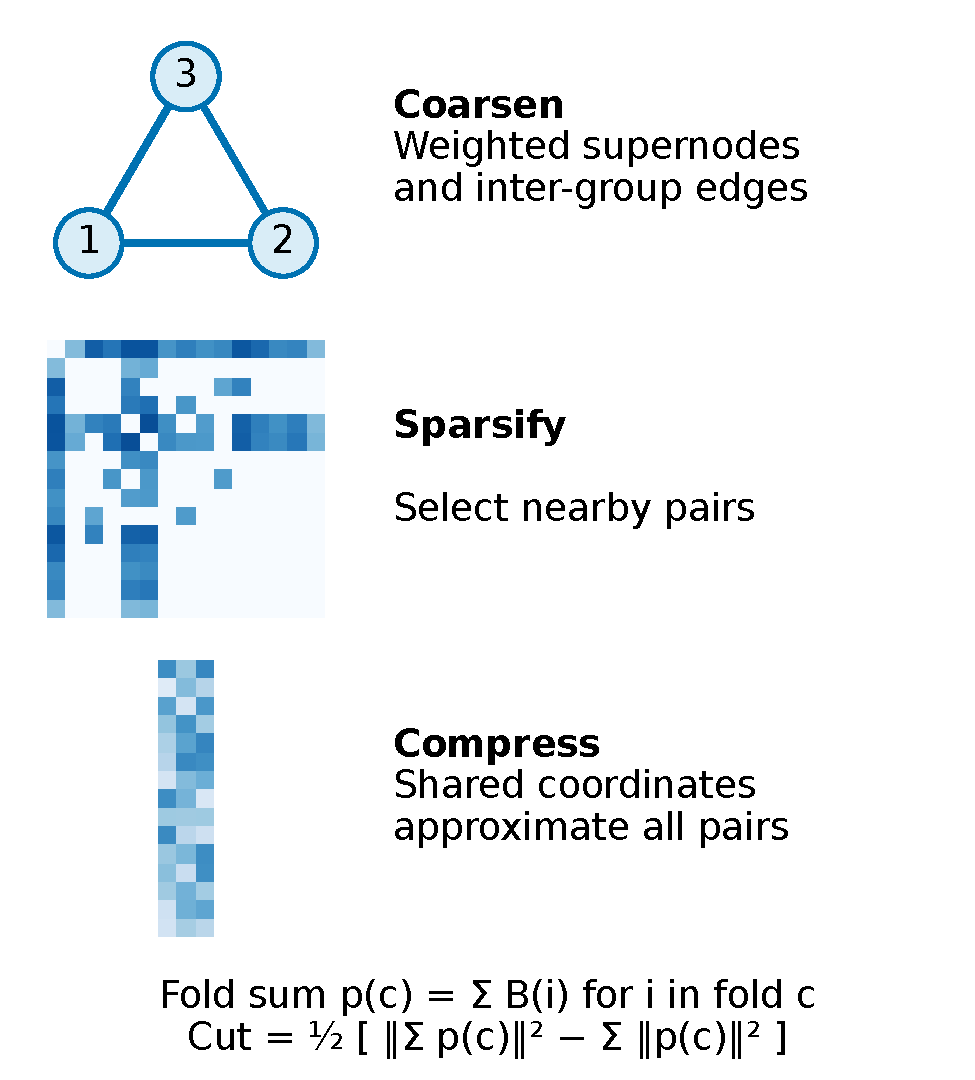
\includegraphics[width=6.5in]{systematic/concept.pdf}
\caption{Representing similarity for split construction. Coarsening replaces
entities with weighted supernodes and retains inter-group connections.
Sparsification selects individual pairwise edges. Low-rank compression
represents similarities through shared coordinates, enabling the fold-sum
identity in Equation~\ref{eq:factor}. The illustrations describe representations,
not interchangeable feasible sets or identical algorithms.}
\label{fig:overview}
\end{figure}
\FloatBarrier

\section{Low-rank similarity splitting}
\label{sec:framework}

\subsection{Objective and compressed representation}

Let $S\in\R^{n\times n}$ be a symmetric, nonnegative, positive-semidefinite
similarity kernel, and let $z_i$ denote entity $i$'s fold. Define the unordered
cross-fold cut and its normalized overlap as
\begin{equation}
 \cut_S(z)=\sum_{i<j}S_{ij}\mathbf{1}[z_i\ne z_j],
 \qquad L_S(z)=\frac{\cut_S(z)}{\sum_{i<j}S_{ij}}.
 \label{eq:cut}
\end{equation}
The denominator is independent of the partition; the diagonal never contributes.
We report the ratio only when its denominator is positive. Nonnegative
similarity is essential to this interpretation. Positive semidefiniteness alone
does not make a signed cosine kernel an overlap measure.

We construct a Nystr\"om factor from $r$ landmarks. If $C$ contains
entity--landmark similarities and $W=U\Lambda U^\top$ is the landmark kernel,
retaining its numerically positive eigenvalues gives
$B=CU_+\Lambda_+^{-1/2}$ and $\widetilde S=BB^\top$.
For fold sums $p_c=\sum_{i:z_i=c}B_i$, the approximate cut is exactly
\begin{equation}
 \cut_{\widetilde S}(z)=
 \frac12\left(\left\|\sum_c p_c\right\|^2-\sum_c\|p_c\|^2\right).
 \label{eq:factor}
\end{equation}
Factor storage and fold-sum construction require $O(nr)$ space and work,
respectively. This identity makes repeated objective evaluation practical
without constructing $\widetilde S$.

At equal fixed fold sizes, minimizing this cut agrees with kernel k-means.
Unequal capacities give a different weighting of within-fold similarity, so
ordinary kernel k-means guarantees do not transfer directly. We distinguish
the approximation of $S$, the quality of the heuristic optimizer, and the
scientific meaning of the selected split. The supplement derives the relevant
identities and conditional error bound.

\subsection{Capacities, optimization and accuracy}

Largest-remainder rounding converts requested proportions into integer targets
summing to $n$. Zero tolerance enforces those targets exactly; positive tolerance
permits a declared two-sided corridor. Seeded restarts alternate fold-sum
calculation with capacity-constrained assignment proposals, accepting proposals
that do not increase the factor objective. A bounded shortlist is refined before
the final candidate is selected. Legal single moves operate within a corridor;
swaps preserve exact counts \citep{fiduccia1982,kernighan1970}.
The standard setting uses four restarts, at most 25 assignment iterations and
two refined candidates. The optimizer remains heuristic.

Rank can be fixed or selected using a bounded accuracy budget. The optional
joint policy grows pair sampling when uncertainty prevents a decision and
grows rank when the estimated error is established as too large or the probe
budget is exhausted. It accounts for all checks over a declared rank--sample
grid and uses a separate final audit. The cut criterion concerns the returned
partition, normalized by the kernel's total absolute off-diagonal mass.
Establishing this tolerance does not certify a uniform approximation over all
partitions or a near-optimal partition. Budget failure is reported explicitly.

\subsection{Controlling strong local relationships}

For integer $p\ge1$, we can factorize the elementwise power $S^{\circ p}$.
The Schur product theorem preserves positive semidefiniteness. Powering reduces
weak similarities relative to strong ones: $0.1^3=0.001$, whereas $0.7^3=0.343$.
If $N_\tau(z)$ counts crossing pairs with similarity at least $\tau>0$, then
$\cut_{S^{\circ p}}(z)\ge\tau^pN_\tau(z)$.
The powered cut consequently provides a soft penalty on strong crossing pairs.
It is distinct from the mean nearest-neighbour evaluation score, and its
approximation requirements must be checked separately.

Grouping restricts which assignments are permitted. We process top-32-neighbour
edges above a threshold in decreasing similarity, merging components subject
to a size cap. A group's factor is the sum of its members' rows; its weight is
their count. Group contraction therefore preserves the factor objective exactly.
The combined molecular setting uses $p=3$, threshold 0.4, and a cap of half the
smallest target fold, with component growth frozen after a cap-blocked merge.

The capacity contract determines what happens when whole groups cannot be packed.
The default count-first policy may dissolve groups and reports that relaxation.
The strict policy preserves every group or reports infeasibility or an unresolved
feasibility check. Neither capped grouping nor a powered objective guarantees
that every pair above the threshold stays within one fold. All reported quality
scores use the original ordinary kernel.

\subsection{Computational scope}

The factor removes quadratic matrix storage, not every source of quadratic
work. Input features still require $O(nd)$ space and can dominate process memory.
Factor construction, assignment sorting and the number of accepted
refinement moves determine runtime. Exact neighbour construction adds quadratic
pairwise arithmetic even when temporary memory is blocked. Plain and combined
settings therefore have separate measured scaling ranges, and exact-count
refinement can cost substantially more than a relaxed corridor. Timing and
memory scopes accompany the measurements.

\FloatBarrier
\section{Results}
\subsection{Compression preserves the ordinary cut, and optimization adds to grouping}

The first question concerns the objective represented by the factor.
Across six full molecular datasets, three seeds and five partitions per factor,
the largest observed rank-256 error is \CurrentPlainFidelity{} of the ordinary
kernel's off-diagonal mass. The corresponding error for the cubed kernel is
\CurrentPowerFidelity{}. At rank 512 these values are
\CurrentPlainHighRankFidelity{} and \CurrentPowerHighRankFidelity{}, respectively
(Figure~\ref{fig:current-fidelity}). Ordinary-kernel fidelity consequently cannot
be transferred to the powered objective. A coarse powered factor can still
produce useful local separation, but that behavior must be measured on the
returned partition rather than inferred from ordinary-kernel accuracy.

\begin{figure}[htbp]
\centering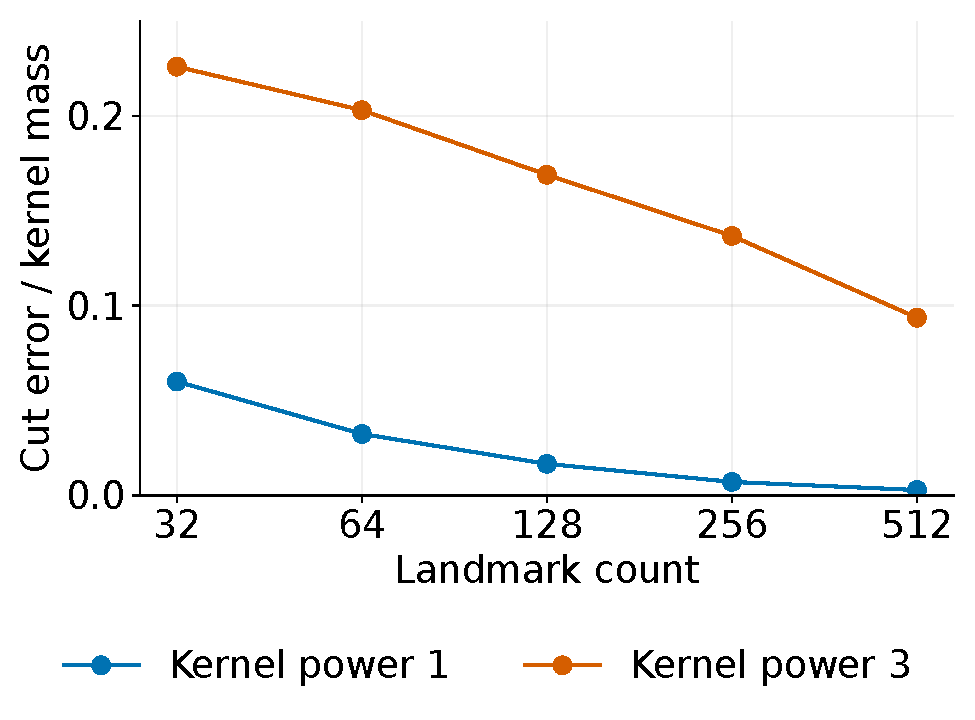
\includegraphics[width=6.5in]{systematic/fidelity.pdf}
\caption{Current-code cut fidelity. Each point is the largest absolute
factor-versus-exact cut difference divided by the corresponding kernel's
off-diagonal mass, over six full datasets, three factor seeds and five
partitions. Each set contains the returned partition and four count-preserving
perturbations. The ordinary and cubed kernels have different denominators.
These are observed cut errors, not uniform approximation guarantees.}
\label{fig:current-fidelity}
\end{figure}

Grouping alone is an incomplete explanation for the method's separation.
With the entities, groups and exact fold counts fixed, factor-space optimization
improves both global overlap and mean nearest-training similarity on all six
datasets, relative to a seeded feasible assignment
(Table~\ref{tab:matched-groups}). Every group is preserved in these controls.
The experiment isolates an improvement available after grouping has already
been chosen; it does not attribute every advantage of the combined pipeline
to compression.

\begin{table}[htbp]\centering
\begin{tabular}{lrr}\toprule
Assignment & Global overlap / random & Mean nearest similarity\\\midrule
Feasible groups & 0.959 & 0.387\\
Groups + ordinary factor & 0.791 & 0.306\\
Groups + cubed factor & 0.745 & 0.292\\
\bottomrule\end{tabular}
\caption{Optimization beyond grouping. Every comparison retains the same entities, constructed groups and exact 80/10/10 counts. Values average six dataset means after averaging three seeds. The factor optimizer starts from the feasible control and preserves every group. Both optimized settings improve both measures on all six datasets. Lower values indicate less overlap.}
\label{tab:matched-groups}\end{table}

\FloatBarrier

Exact references distinguish approximation from optimization more directly.
On twenty 12-entity instances, we enumerate 2,970 admissible ungrouped
assignments and thirty assignments with paired entities as indivisible groups.
Even with all twelve landmarks, the heuristic has nonzero optimization gaps
on some ungrouped instances: the largest gaps are 0.0132 and 0.0408 of kernel
mass for the ordinary and cubed kernels. The grouped full-landmark cases reach
their enumerated optima in this small suite. Increasing rank can therefore
remove approximation error while leaving a separate optimization error.
The complete decomposition and accuracy--cost controls appear in the supplement.

\FloatBarrier
\subsection{Dense overlap and analogue exposure give different quality--cost choices}

The ordinary factor directly targets distributed overlap. Its mean global
score is \CurrentPlainGlobal{}, compared with \CurrentGraphGlobal{} for the
top-32 graph, after averaging seeds within each dataset.
The combined setting reduces nearest-training exposure relative to the plain
setting, while the top-32 graph achieves lower mean exposure than the combined
setting (\CurrentGraphNearest{} versus \CurrentCombinedNearest{}).
Changing graph degree also changes the available trade-off
(Figure~\ref{fig:current-quality}). These outcomes support choosing a
representation and objective for a specified boundary rather than expecting
one method ordering for every separation criterion.

\begin{figure}[htbp]
\centering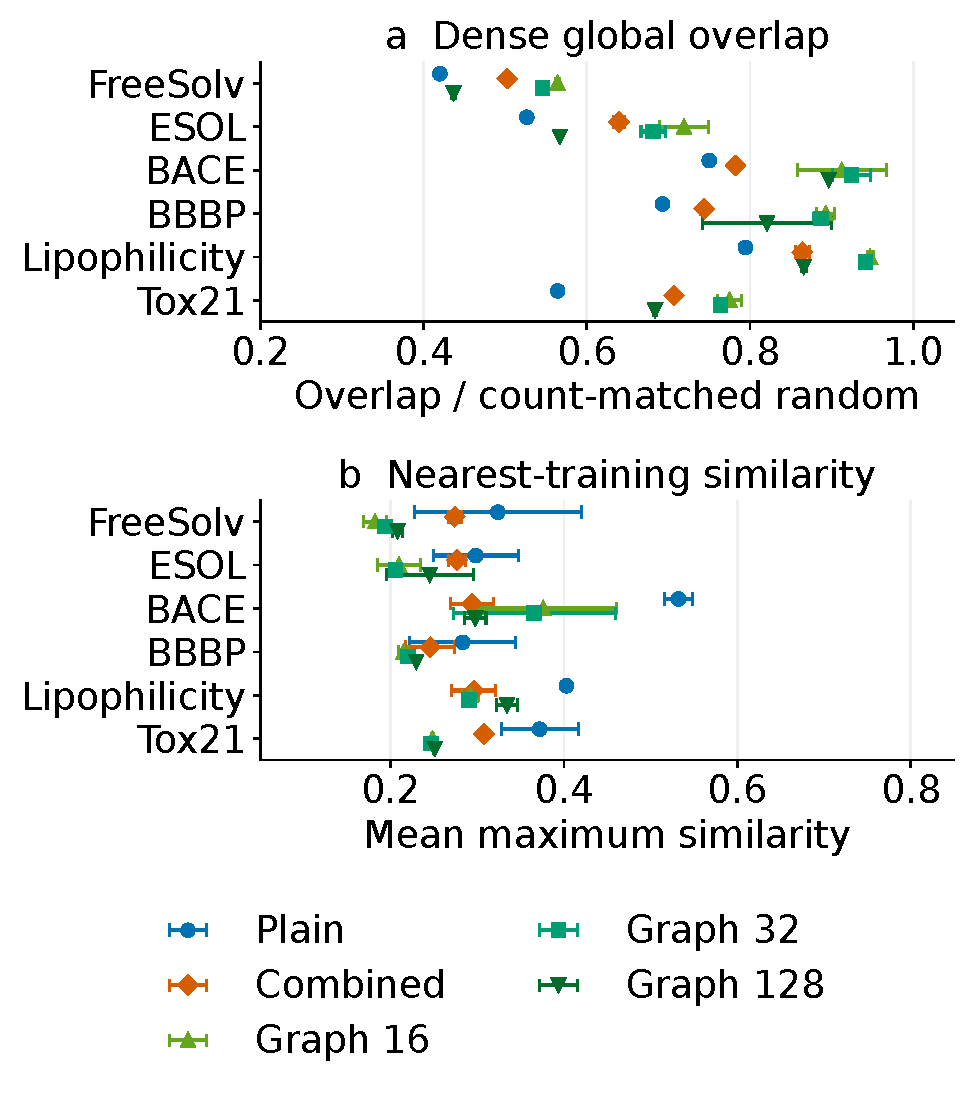
\includegraphics[width=6.5in]{systematic/quality.pdf}
\caption{Global and local quality for six full molecular datasets.
The primary global score is normalized by the analytic random expectation at
the actual counts; the local score is mean test-to-training maximum similarity.
Points average three split seeds and bars show their standard deviations.
All methods retain the same input entities and use a 1\% count corridor.
Graph labels identify ordinary pairwise degrees; graph construction and any
count repair are included in its runtime. All scores use the original ordinary
Tanimoto kernel. Lower values indicate less overlap.}
\label{fig:current-quality}
\end{figure}

DataSAIL provides the closer dense-objective comparison and reveals the
importance of admissible partitions. Sixteen of its twenty-four prespecified
configurations return assignments; eight report infeasibility under their
cluster and capacity settings. At exactly matched native counts, entity-level
low rank has mean global score \CurrentMatchedGlobal{}, versus
\CurrentNativeGlobal{} for DataSAIL. Requiring low rank to preserve the groups
passed to DataSAIL's solver changes its mean to
\CurrentMatchedGroupsGlobal{}, eliminating that average quality advantage.
These summaries weight the four datasets equally after averaging their
configurations.

Matching counts alone thus leaves a material difference in constraints.
Matching groups also leaves a distinction between linked cluster similarities
and sums over entity-level similarities, as well as different optimizers.
The comparison does not establish that compression solves an identical
optimization problem better. It establishes an economical way to construct
entity-level dense-overlap splits, with the consequences of additional
indivisibility constraints made visible. The supplement reports all native
outcomes, timings, group-preserving controls and memory profiles.

\FloatBarrier
\subsection{Exact capacities have a measurable computational cost}

At 100,000 ChEMBL fingerprints on two CPU cores, the median plain split-call
time is \CurrentExactCpuSeconds{} seconds with exact counts and
\CurrentCorridorCpuSeconds{} seconds with a 1\% corridor.
The inputs, rank and restart settings are otherwise matched.
The difference reflects the cost of feasible refinement, including the use of
swaps at exact capacities (Figure~\ref{fig:current-scaling}).
Linear factor storage therefore does not imply the same runtime at different
capacity tolerances.

On lambda13, the current plain implementation partitions two million
fingerprints in a median \CurrentLargeCpuSeconds{} seconds using 32 CPU cores,
with peak process RSS of \CurrentLargeCpuMemory{} GiB.
All three cases retain all entities and satisfy the declared 1\% corridor.
This is a separate hardware configuration from the paired two-core comparison;
the difference is not interpreted as an algorithmic speedup.

\begin{figure}[htbp]
\centering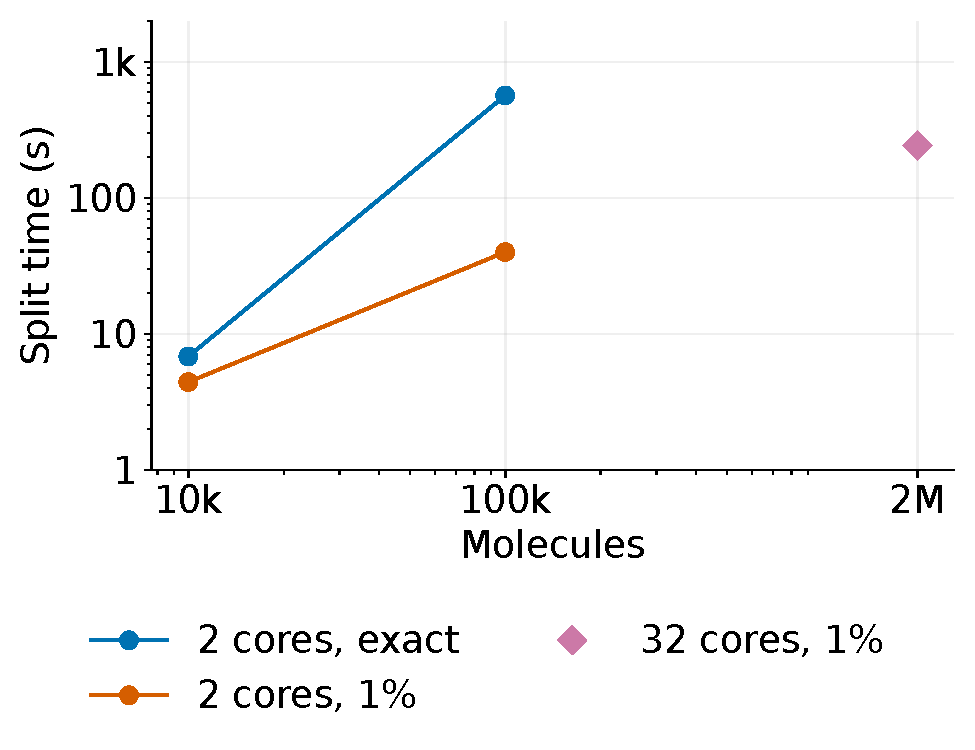
\includegraphics[width=6.5in]{systematic/cpu_scaling.pdf}
\caption{Current-code plain split-call time on nested ChEMBL samples, using
rank 256, four restarts and two refined candidates. Two-core cases run on lambda2;
the separate 32-core point runs on lambda13. Points are medians of completed cases.
Warm-up, feature loading and independent auditing
are outside the split clock. The full case inventory, including end-to-end
budget failures and the distinct combined-setting range, appears in the
supplement. An end-to-end failure is not assigned a split-call runtime.}
\label{fig:current-scaling}
\end{figure}

The large-data protocol checks quality as well as computational cost.
For every completed 100,000- and two-million-entity plain case, the independently
sampled returned-cut error interval has an upper endpoint below 0.008 of ordinary
kernel mass. Uniformly sampled test queries are also compared with every
training entity, rather than a subsampled training reference.
At two million entities, mean nearest-training similarity is
\CurrentLargeNearest{} across the three sets of sampled queries, showing that
low global overlap does not remove close-analogue exposure.
Sample sizes and conservative query-sampling intervals accompany the results.
The earlier v0.1 H100 measurements remain archival evidence and are not used
as timings of the current implementation.

\FloatBarrier
\subsection{Split usefulness depends on the transfer task}

Independent cohorts give a direct test of what an evaluation boundary predicts.
In the synthetic family model, random splitting identifies the better model
for known-family interpolation in all twenty generated instances, but identifies
the better model for new-family transfer in none. The combined split shows the
reverse pattern: agreement in all twenty new-family instances and none of the
interpolation instances. Plain splitting lies between these outcomes
(Figure~\ref{fig:current-deployment}).

\begin{figure}[htbp]
\centering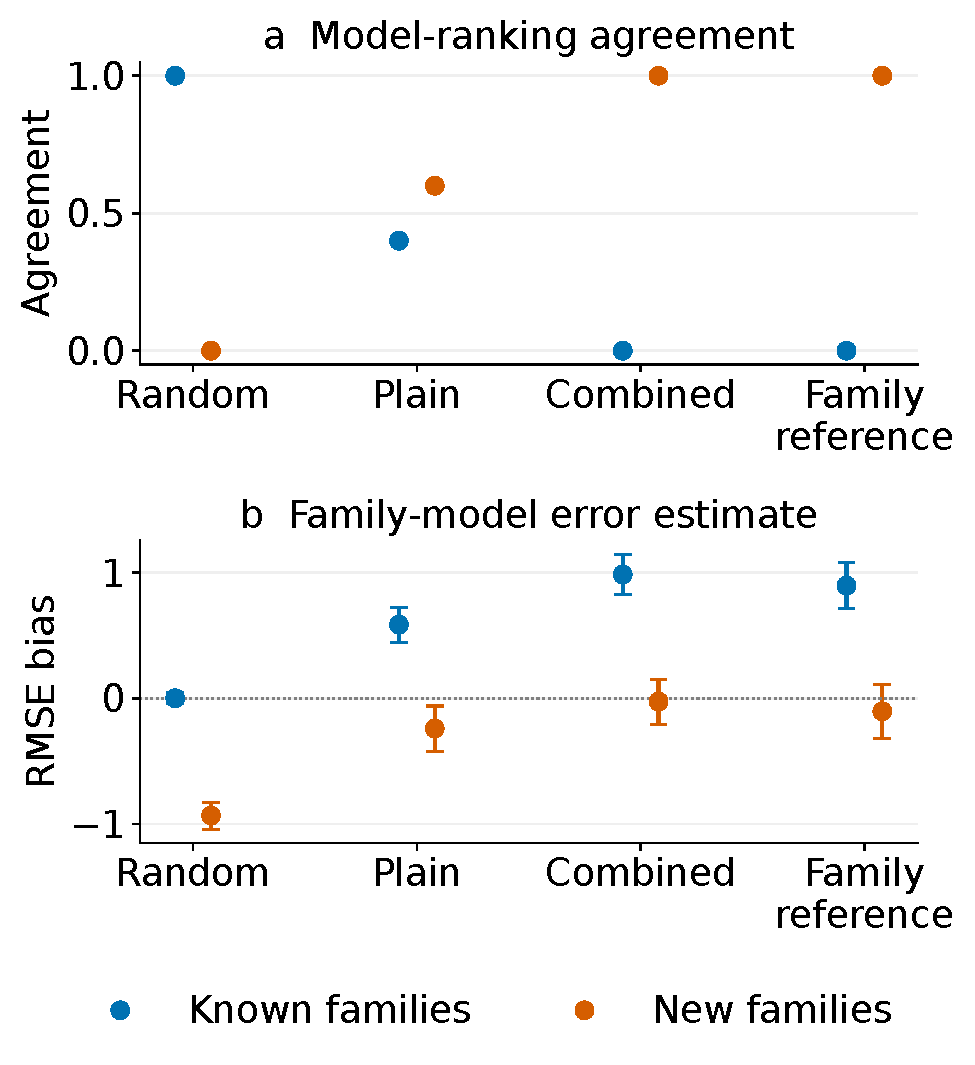
\includegraphics[width=6.5in]{systematic/deployment.pdf}
\caption{Evaluation boundaries for two transfer tasks in twenty synthetic
instances. (a) Agreement of held-out and independent-cohort model rankings.
(b) RMSE bias for the family-sensitive model; negative values are optimistic.
Bars are descriptive 95\% bootstrap intervals over instances.
Known-family cohorts condition on families present in training.
The family reference uses generator identities, and invariant ridge receives
the stable features. This mechanism test supplies no prospective validation.}
\label{fig:current-deployment}
\end{figure}

The direction of error is as relevant as the ranking. Random evaluation is
optimistic about the family-sensitive model on the new-family cohort, whereas
the combined split is pessimistic about that model's interpolation performance.
Stronger separation is useful when it matches the intended transfer boundary.
Its lower held-out score alone does not make it a more realistic test.

An earlier-release assay study illustrates a related risk in real molecular
data. Across ten prespecified external assays, the combined setting gives
mean random-forest ROC-AUC \ExtCombinedRF{}. A label-balance sensitivity intervention at
unchanged counts raises this to \ExtCombinedBalancedRF{}.
The intervention also changes structural composition and may break groups,
so it cannot isolate a causal contribution of label proportions.
These archival results demonstrate why target composition and absolute
predictive scores should accompany similarity measures. They supply no
observed future outcomes against which to validate a deployment claim.

\FloatBarrier

\section{Discussion}

Low-rank coordinates make dense overlap available as a split-design objective
at specified fold capacities. The useful contribution is the combination of a
compact objective, explicit constraints and auditable trade-offs. The
matched-group controls show that optimization contributes beyond forming groups.
The DataSAIL controls also show why feasible sets matter: an advantage observed
at matched counts can disappear when indivisible clusters are matched as well.
These comparisons support a practical computational framework without
establishing universal superiority in partition quality.

Global and local overlap describe different evaluation boundaries. The plain
factor favors reducing distributed similarity mass. Powers and groups can
strengthen analogue separation while changing global overlap, approximation
accuracy and cost. A sparse graph can provide stronger local separation for a
given configuration. Choosing among these outcomes requires specifying which
relationships should transfer from training to evaluation. The synthetic
independent-cohort experiment demonstrates that both optimistic and pessimistic
model-selection errors can result from choosing the wrong boundary.

A practical evaluation should state its intended transfer task, capacities,
representation and retention policy before examining final model outcomes.
It should then report global overlap, nearest-training exposure and target
composition together. The software also permits fold-pair weights when only
particular evaluation boundaries matter; the primary benchmarks use the
ordinary all-fold objective. Label-informed changes belong to declared benchmark
design or sensitivity analysis, with a separate final evaluation.

Several limits remain. The datasets are convenience samples, and conclusions
about molecular separation depend on the fingerprint representation.
A small returned-cut error leaves optimizer suboptimality unresolved.
Powering can require substantially more rank, and strict whole-group capacities
can be infeasible. Storage scaling alone does not establish fast construction
at every size or tolerance. The synthetic invariant model receives the
generative stable features, making it a mechanism test rather than evidence of
prospective performance on real projects. Real deployment validation requires
independently specified project tasks and genuine dated outcomes; simulated
temporal labels cannot supply those outcomes.

\section{Conclusion}

Compressed fold sums support capacity-controlled similarity splitting while
exposing approximation and optimization limits. Their scientific value is in
constructing an evaluation boundary whose relation to the intended transfer
task can be examined explicitly.

\clearpage
\section{Methods}
\label{sec:methods}

\subsection{Implementation, data and scoring}

Primary numerical experiments use the pinned v0.2.0.dev3 implementation.
The six full molecular datasets are FreeSolv, ESOL, BACE, BBBP, Lipophilicity
and Tox21 \citep{wu2018moleculenet}. Radius-two Morgan fingerprints have 1024 bits,
with binary Tanimoto similarity
\citep{rogers2010fingerprints,ralai2005}.
Structural optimization uses no response values and retains every successfully
featurized input entity. Raw-input, feature, source and assignment hashes identify
the exact observations. Earlier-release experiments are separated in the
supplement, including the eleven-dataset molecular comparison, two
composition-descriptor materials checks, neural-model reuse and external assays.

For actual counts $n_c$, the random expectation of the global fraction is
\begin{equation}
 \mathbb{E}[L_S]=1-\frac{\sum_c n_c(n_c-1)}{n(n-1)}.
 \label{eq:random}
\end{equation}
The primary global score is $L_S/\mathbb{E}[L_S]$.
The primary local score is the raw mean
$\nnl=|T|^{-1}\sum_{i\in T}\max_{j\in R}S_{ij}$, where $T$ is the test fold
and $R$ the training fold. Lower values indicate less overlap.
The six-dataset comparison scores all pairs and all test-to-training neighbours.
Independent NumPy calculations check the saved global and local scores.
Threshold ramps and alternative fingerprints are supporting diagnostics;
their definitions are kept separate from the primary local score.

\subsection{Controls and established comparators}

The group mechanism study uses three seeds and exact 80/10/10 counts.
For each dataset and seed, a single set of capped groups is fixed.
A seeded capacity-feasible assignment constructed without factor values serves
as the control. Ordinary and cubed factors are optimized from that incumbent
while preserving every group. Exact small-instance references use twenty
12-entity binary datasets, counts 8/2/2, powers one and three, and landmark counts
2, 4, 8 and 12. Enumerating all feasible assignments measures approximation and
optimization gaps separately, both without groups and with pairs as indivisible
groups.

DataSAIL is the established comparator for reducing dense cross-fold similarity
\citep{joeres2025datasail,joeres2026datasailaddendum}.
An ordinary weighted k-nearest-neighbour graph tests the alternative of selecting
pairs rather than compressing their similarities. We use Mt-KaHyPar's Graph API,
QUALITY preset and CUT objective \citep{gottesburen2024}, with degrees
16, 32 and 128. Exact top-k construction, safe integer weight encoding,
partitioning and any lower/upper count repair are included in its split clock.
Native and repaired assignments are retained separately.

The six-dataset graph and low-rank comparison uses three split seeds,
8:1:1 proportions and tolerance 0.01. DataSAIL 1.3.0 uses C1e with SCIP on
FreeSolv, ESOL, BACE and BBBP. Its prespecified grid combines cluster counts
$9$, $\max(9,\lfloor n/50\rfloor)$ and $\max(9,\lfloor n/20\rfloor)$ with
solver budgets of 60 and 300 seconds, $\delta=0.1$ and $\epsilon=0.01$.
Every native assignment receives an entity-level low-rank control at its exact
counts and another control preserving the groups passed to its native solver.
Equal groups do not make DataSAIL's linked cluster similarities identical to
the entity-level dense objective. Solver-reported infeasibility remains a
reported outcome rather than an imputed score.

Lo-Hi, UMAP/Ward, scaffold and Butina comparisons address additional retention
or grouping contracts and remain in the explicitly versioned archival studies
\citep{steshin2023lohi,hernandez2023clustering,guo2025umap,bemis1996frameworks,butina1999clustering}.
Their retained subsets and realized counts accompany the comparisons.
They are not silently substituted for equal-constraint controls.

\subsection{Fidelity, accuracy budgets and computation}

Full-kernel fidelity uses six datasets, three factor seeds, five landmark counts
and powers one and three. For each setting, we evaluate the current returned
partition and four count-preserving perturbations against an independent full
NumPy Tanimoto kernel. Absolute cut error is divided by the off-diagonal mass
of the kernel at that power. This yields 900 comparisons, not 900 independent
datasets.

Joint accuracy selection uses ranks 32--512, a cut tolerance of 0.05 and probe
counts up to 32,768. For $R$ rank stages and $Q$ pair-count stages, selection
checks allocate failure probability $0.025/(RQ)$ each. An independent final
audit uses failure probability 0.025. A union bound gives at least 95\%
coverage for selection and final auditing together under the bounded-sampling
assumptions. Fixed-size probe grids use the same policy with equal initial and
maximum pair counts. Pair counts, allocation decisions and unestablished
tolerances remain in the diagnostics. Model test outcomes do not select rank
or audit budgets.

CPU comparisons use disjoint two-core affinities, two-thread native pools and
hidden CUDA devices. Wall-clock split times include factorization, assignment,
refinement and any method-specific graph or clustering work; feature loading,
imports and quality scoring are excluded. A small common low-rank warm-up is
reported separately. Native memory profiles record fresh-process peak RSS before
scoring or matched controls. They include input arrays and framework overhead.

Scaling uses nested samples of packed 2048-bit ChEMBL 37 fingerprints
\citep{chembl37}, four
restarts, two refined candidates, rank 256, and exact or 1\% capacity corridors.
The plain and combined settings are measured separately.
Independent large-data audits use 262,144 uniform pair draws and up to
128 uniformly sampled test queries, each evaluated against the complete training
fold. A conservative bounded-mean interval describes query-sampling uncertainty.
End-to-end case-budget failures include loading and auditing and are
distinguished from split-call timings.

\subsection{Independent-cohort experiment and uncertainty}

A synthetic regression generator supplies fifty observed families with forty
entities each. Responses combine a linear function of four stable features,
an independent family effect and observation noise. Nonnegative cosine
features encode family identity and a weaker continuous signal.
Two fixed models represent different inductive assumptions: five-neighbour
regression on the full representation and ridge regression supplied with the
generative stable features. The latter is an explicitly privileged invariant
reference. Plain and combined splitting use rank 128; the plain cosine kernel
uses its exact finite feature map when available.

For twenty prespecified generative seeds, each split retains 1600 training,
200 validation and 200 test entities. Models are fitted on training labels only.
Their held-out RMSE and ranking are compared with independently drawn observations
from families present in that training set and with observations from fifty
new families. The family-reference split uses the generator's known family
identities and is a mechanism control. Cohort outcomes never enter split
construction. This experiment contains no real experiment dates or prospective
application evidence.

Summaries average seeds within each dataset before averaging datasets.
DataSAIL configuration comparisons likewise average configurations within
datasets first. Descriptive bootstrap intervals resample dataset means or
independent synthetic instances, using 10,000 draws and seed 31415.
Seeds, models and perturbations of the same dataset are not treated as independent
projects. All method settings, realized counts, native outcomes and per-case
timing and memory scopes are retained.

\section*{Data and code availability}

Code, manuscript sources, compiled PDFs, study manifests and saved assignments
are available in the
\href{https://github.com/Ray16/PALM/tree/lowrank-v0.2.0-review-20261026/publications/lowrank_2026}{versioned PALM manuscript release}.
The primary numerical implementation is pinned to commit \texttt{f7e0866};
the delivered source and environment records identify later documentation and
manuscript changes and reproduction adapters. Public-input recipes and checksums accompany the records.
The earlier
\href{https://github.com/Ray16/PALM/tree/lowrank-v0.1.0-review-20261021-r2/publications/lowrank_2026}{v0.1 review release}
preserves the archival experiments. MoleculeNet, ChEMBL, QMOF, Materials Project
and SIMPD inputs retain their original attribution and terms.

% Author-supplied information is intentionally pending in this technical draft.
\section*{Author contributions}
Pending author-supplied CRediT statement.

\section*{Funding}
Pending author-supplied funding statement.

\section*{Competing interests}
Pending author-supplied competing-interest statement.

\section*{Acknowledgements and use of AI tools}
OpenAI Codex and Anthropic Claude assisted with code development and review,
analysis and manuscript preparation. The authors are responsible for the
scientific claims, references and final submitted manuscript.
\bibliographystyle{unsrtnat}
\bibliography{references}
\end{document}
